\documentclass[10pt]{article}
\usepackage[UTF8]{ctex}

\usepackage[utf8]{inputenc} % allow utf-8 input
\usepackage{amsthm}  
\usepackage{amsmath,amscd}
\usepackage{amssymb,array}
\usepackage{amsfonts,latexsym}
\usepackage{graphicx,subfig,wrapfig}
\usepackage{times}
\usepackage{psfrag,epsfig}
\usepackage{verbatim}
\usepackage{tabularx}
\usepackage[pagebackref=true,breaklinks=true,letterpaper=true,colorlinks,bookmarks=false]{hyperref}
\usepackage{cite}
\usepackage{algorithm}
\usepackage{multirow}
\usepackage{caption}
\usepackage{algorithmic}
%\usepackage[amsmath,thmmarks]{ntheorem}
\usepackage{listings}
\usepackage{color}
\usepackage{bm}



\newtheorem{thm}{Theorem}
\newtheorem{mydef}{Definition}

\DeclareMathOperator*{\rank}{rank}
\DeclareMathOperator*{\trace}{trace}
\DeclareMathOperator*{\acos}{acos}
\DeclareMathOperator*{\argmax}{argmax}


\renewcommand{\algorithmicrequire}{ \textbf{Input:}}     
\renewcommand{\algorithmicensure}{ \textbf{Output:}}
\renewcommand{\mathbf}{\boldsymbol}
\newcommand{\mb}{\mathbf}
\newcommand{\matlab}[1]{\texttt{#1}}
\newcommand{\setname}[1]{\textsl{#1}}
\newcommand{\Ce}{\mathbb{C}}
\newcommand{\Ee}{\mathbb{E}}
\newcommand{\Ne}{\mathbb{N}}
\newcommand{\Se}{\mathbb{S}}
\newcommand{\norm}[2]{\left\| #1 \right\|_{#2}}

\newenvironment{mfunction}[1]{
	\noindent
	\tabularx{\linewidth}{>{\ttfamily}rX}
	\hline
	\multicolumn{2}{l}{\textbf{Function \matlab{#1}}}\\
	\hline
}{\\\endtabularx}

\newcommand{\parameters}{\multicolumn{2}{l}{\textbf{Parameters}}\\}

\newcommand{\fdescription}[1]{\multicolumn{2}{p{0.96\linewidth}}{
		
		\textbf{Description}
		
		#1}\\\hline}

\newcommand{\retvalues}{\multicolumn{2}{l}{\textbf{Returned values}}\\}
\def\0{\boldsymbol{0}}
\def\b{\boldsymbol{b}}
\def\bmu{\boldsymbol{\mu}}
\def\e{\boldsymbol{e}}
\def\u{\boldsymbol{u}}
\def\x{\boldsymbol{x}}
\def\v{\boldsymbol{v}}
\def\w{\boldsymbol{w}}
\def\N{\boldsymbol{N}}
\def\X{\boldsymbol{X}}
\def\Y{\boldsymbol{Y}}
\def\A{\boldsymbol{A}}
\def\B{\boldsymbol{B}}
\def\y{\boldsymbol{y}}
\def\cX{\mathcal{X}}
\def\transpose{\top} % Vector and Matrix Transpose

%\long\def\answer#1{{\bf ANSWER:} #1}
\long\def\answer#1{}
\newcommand{\myhat}{\widehat}
\long\def\comment#1{}
\newcommand{\eg}{{e.g.,~}}
\newcommand{\ea}{{et al.~}}
\newcommand{\ie}{{i.e.,~}}

\newcommand{\db}{{\boldsymbol{d}}}
\renewcommand{\Re}{{\mathbb{R}}}
\newcommand{\Pe}{{\mathbb{P}}}

\hyphenation{MATLAB}

\usepackage[margin=1in]{geometry}

\begin{document}
	
\title{	Numerical Optimization, 2020 Fall\\Homework $4$}
\date{Due on 14:59, Oct. 15, 2020\\}
\maketitle

%%%%%--------------------

$\bm{1}.$ 请按要求写出下列线性规划问题对应的对偶问题.
\begin{itemize}
	\item[$(1)$] 请参考Lecture $5$提供的原-对偶表格法, 写出如下问题对应的对偶问题并使用\textbf{图解法}求解.~\textcolor{red}{[15pts]}
	\begin{equation}
		\begin{array}{ll}
			\min & 12 x_{1}+8 x_{2}+16 x_{3}+12 x_{4} \\
			\text { s.t. } & -2 x_{1}-x_{2}-4 x_{3} \leq -2 \\
			& -2 x_{1}-2 x_{2}-4 x_{4} \leq -3 \\
			& x_{i} \geq 0, \quad i=1, \cdots, 4.
		\end{array}
	\end{equation}
	\textbf{解}\\
	根据表格我们写出对应的对偶问题
	\begin{equation}
		\begin{array}{ll}
			\min & -2p_1-3p_2 \\
			\text { s.t. } & -2p_1-2p_2\le 12 \\
			& -p_1-2p_2\le 8 \\
			& -4p_1\le 16 \\
			& -4p_2\le 12 \\
			& p_1,p_2\le 0
		\end{array}
	\end{equation}
	\begin{figure}[h!]
	\centering
	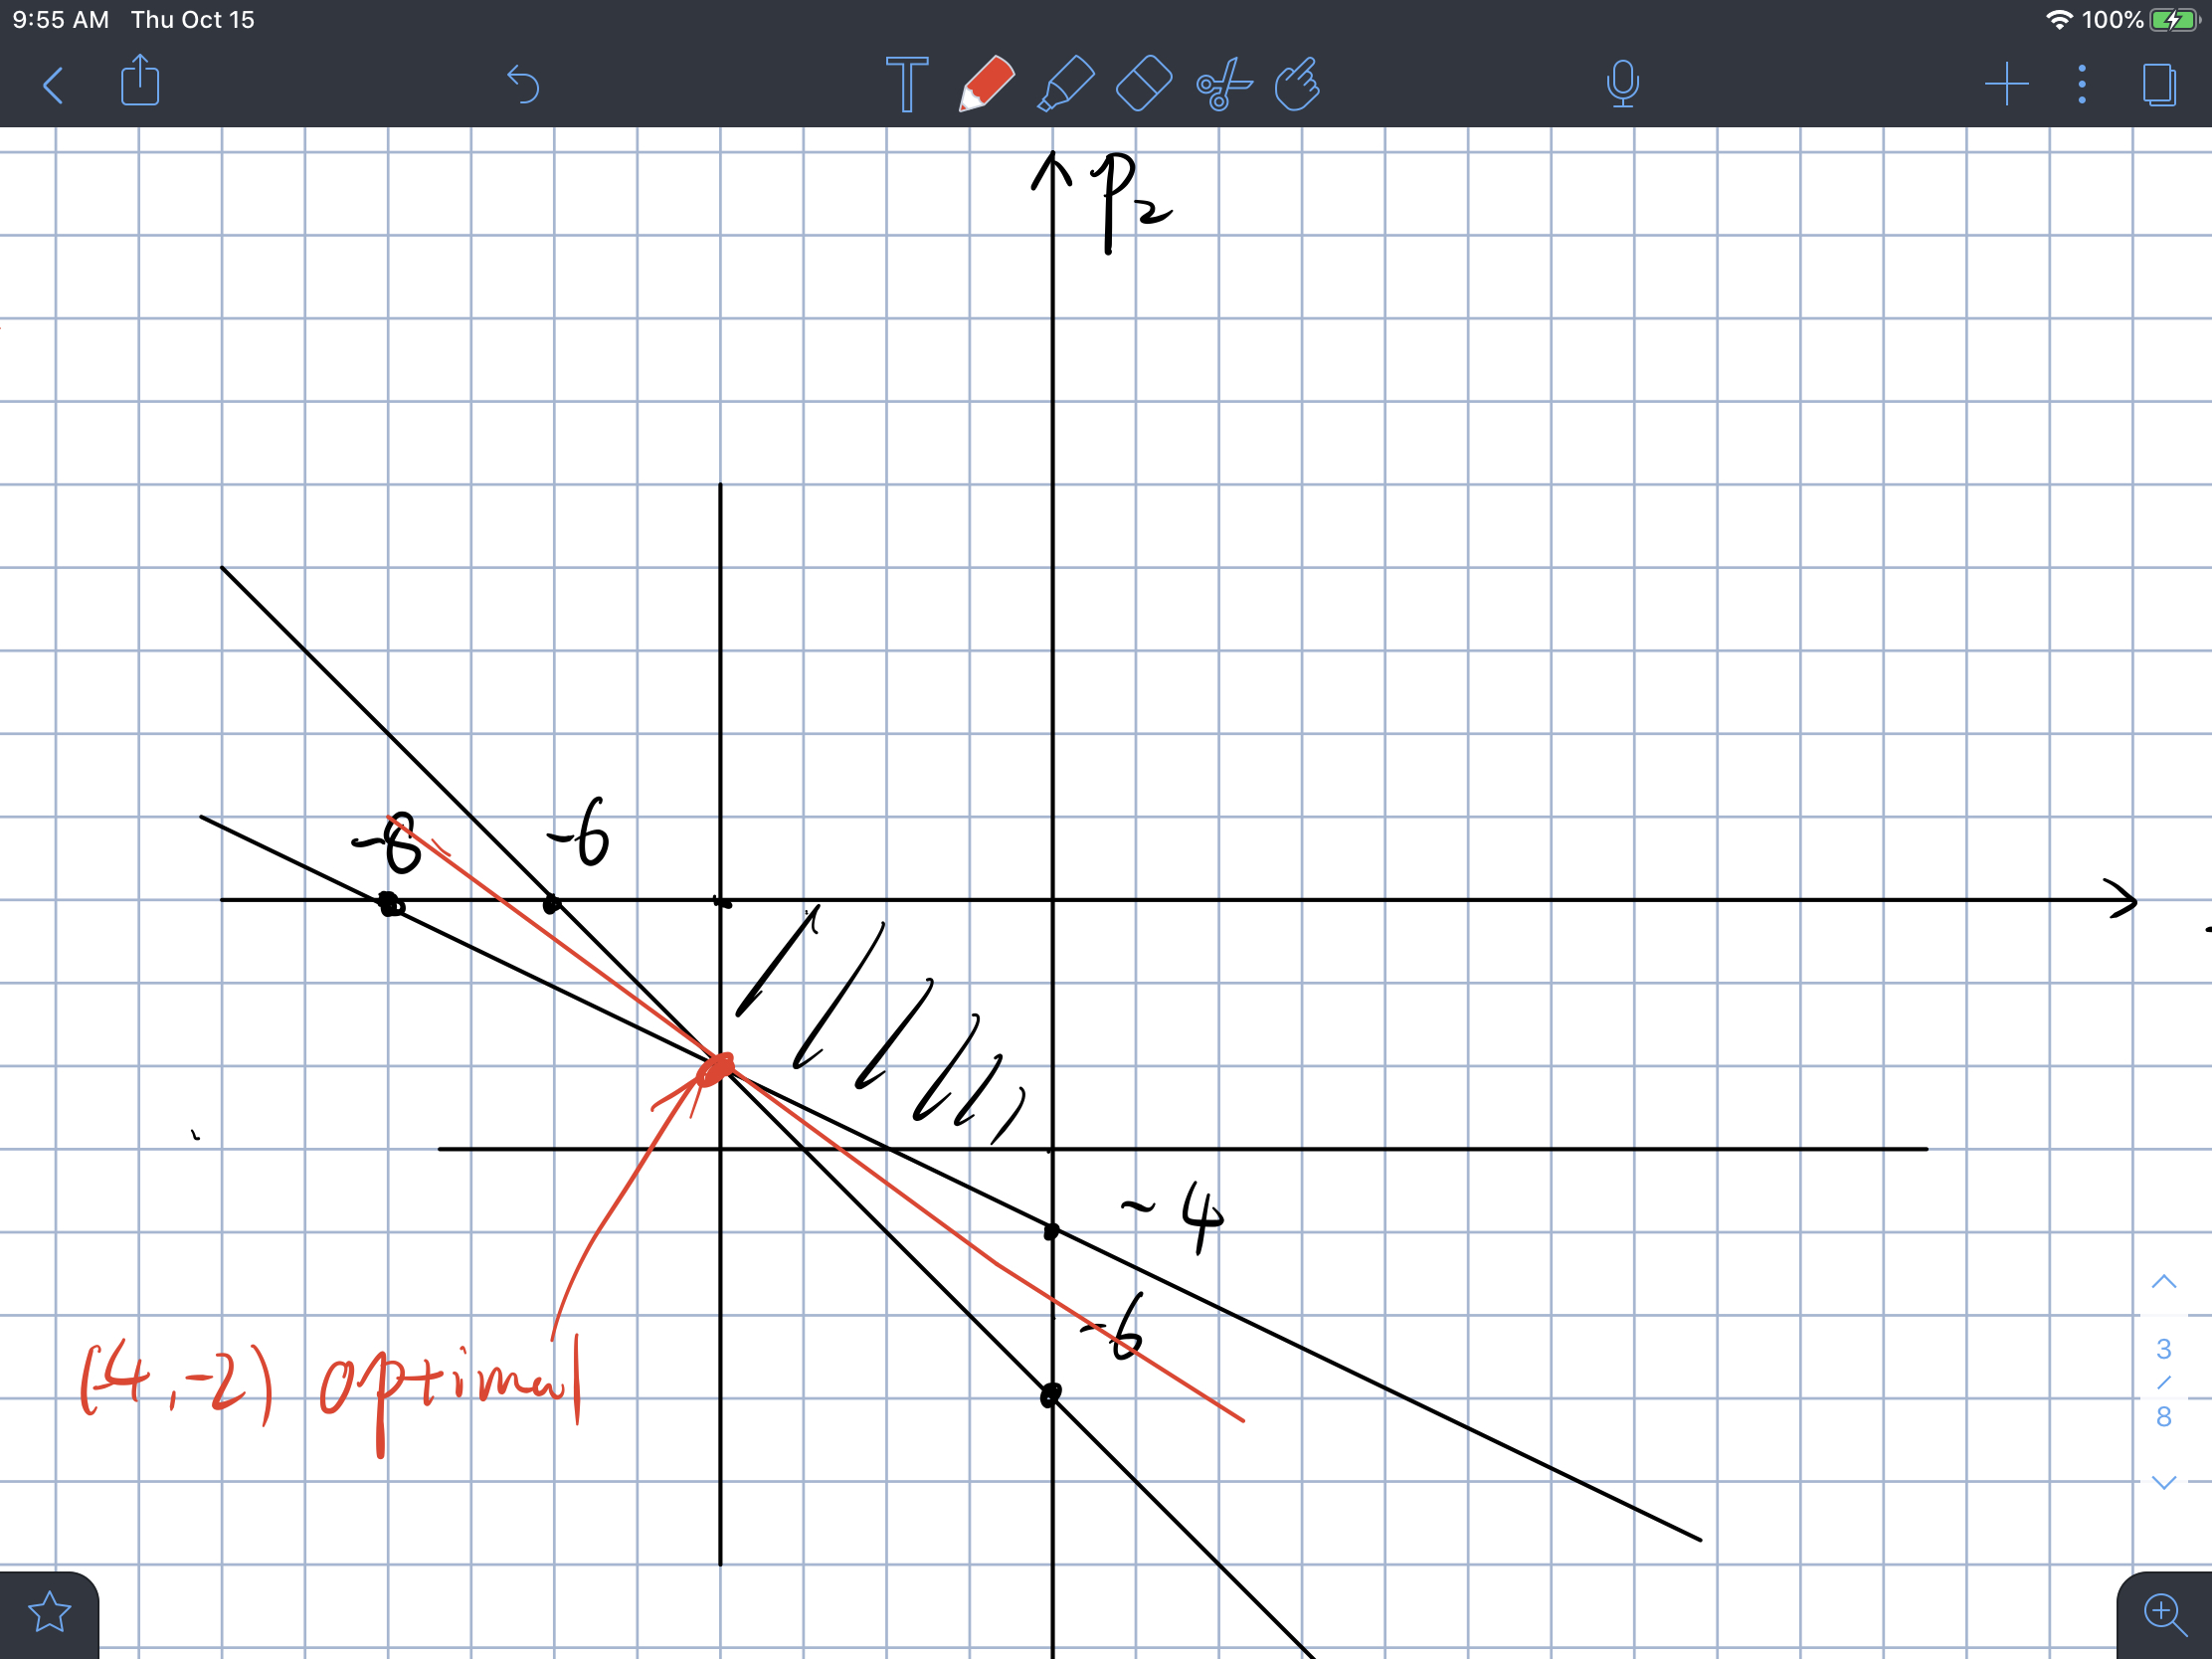
\includegraphics[width=3in]{fig2.jpeg}
	\end{figure}\\
	解得$p_1=-4,p_2=-2$,最优值为14。
	\item[$(2)$] 请使用Lagrange方法写出如下问题对应的对偶问题.~\textcolor{red}{[10pts]}
	\begin{equation}
		\begin{array}{ll}
			\min & x_{1} - x_{2} \\
			\text { s.t. } & 2 x_{1} + 3 x_{2} - x_{3} + x_{4} \leq 0 \\
			& 3 x_{1} + x_{2}  + 4 x_{3} - 2 x_{4} \geq 3 \\
			& -x_{1} - x_{2} + 2 x_{3} + x_{4} = 6\\
			& x_1 \leq 0\\
			& x_{2}, x_{3} \geq 0.
		\end{array}
	\end{equation}
	\textbf{解}\\
	首先写出拉格朗日函数
	\begin{align*}
		L(x,\lambda) &= x_1-x_2+\lambda_1(2x_1+3x_2-x_3+x_4)+\lambda_2(-3x_1-x_2-4x_3+2x_4+3)\\
		&+\lambda_3(-x_1-x_2+2x_3+x_4-6)+\mu_1x_1-\mu_2x_2-\mu_3x_3\\
		&=(1+2\lambda_1-3\lambda_2-\lambda_3+\mu_1)x_1+(-1+3\lambda_1-\lambda_2-\lambda_3-\mu_2)x_2\\
		&+(-\lambda_1-4\lambda_2+2\lambda_3-\mu_3)x_3+(\lambda_1+2\lambda_2+\lambda_3)x_4+3\lambda_2-6\lambda_3\\
		&\lambda_1,\lambda_2\ge 0,\lambda_3\, free, \mu_1,\mu_2,\mu_3\ge 0
	\end{align*}
	因此我们写出对偶问题
	\begin{equation}
		\begin{array}{ll}
			\min & 3\lambda_2 - 6\lambda_3 \\
			\text { s.t. } & 2\lambda_1-3\lambda_2-\lambda_3\le -1 \\
			& 3\lambda_1-\lambda_2-\lambda_3\ge 1\\
			& -\lambda_1-4\lambda_2+2\lambda_3\ge 0\\
			& \lambda_1+2\lambda_2+\lambda3= 0\\
			& \lambda_1,\lambda_2\ge 0.
		\end{array}
	\end{equation}
\end{itemize}

$\bm{2}.$ 考虑如下的两阶段法中第一阶段的辅助问题
\begin{equation}\label{eq: Auxiliary}
	\begin{aligned}
		\min_{\substack{\bm{x}\in \mathbb{R}^{n}\\\bm{y}\in\mathbb{R}^{m}}}~\quad&\sum_{i=1}^{m}y_i\\
		\textrm{s.t.}~\quad&\bm{A}\bm{x} + \bm{y}= \bm{b}\\
		&\bm{x}\geq \bm{0}, \bm{y} \geq \bm{0}
	\end{aligned}
\end{equation}
其中~$\bm{A}\in\mathbb{R}^{m\times n}$, $\bm{c}\in\mathbb{R}^{n}$ 和 $\bm{b}\in\mathbb{R}^{m}$给定.
\begin{itemize}
	\item[$(1)$] 写出问题~\eqref{eq: Auxiliary}~的对偶问题.~\textcolor{red}{[15pts]}\\
	\textbf{解}\\
	x,y为优化变量,根据原-对偶表格可得
	\begin{equation}
		\begin{aligned}
			\min_{\substack{\bm{p}\in \mathbb{R}^{m}}}~\quad&\sum_{i=1}^{m}p_ib_i\\
			\textrm{s.t.}~\quad& \bm{p}^TA \le 0\\
			&\bm{p}^T\le \bm{1}^T
		\end{aligned}
	\end{equation}
	\item[$(2)$] 对于上述问题$(1)$中得到的对偶问题, 请问它有最优解吗?请给出充分的理由.~\textcolor{red}{[15pts]}\\
	\textbf{解}\\
	有最优解,原因如下。首先我们考虑原问题的最优解是否存在,由于$\bm{x}=0,\bm{y}=b$是原问题的一个基本可行解(b在两阶段法中会被处理为非负,非负基本解即为基本可行解),因此根据线性规划基本定理,原问题必定存在一个最优解在基本可行解中。在此基础上,根据强对偶定理:原问题有最优解能得出对偶问题也有最优解,并且最优值相等,因此我们得到$(1)$中得到的对偶问题有最优解。
\end{itemize}


$\bm{3}.$ 
如图~\ref{fig: thm}~示.  请解释: 为什么该定理成立? (\textcolor{red}{提示: 利用强对偶定理.})~\textcolor{red}{[15pts]}
\begin{figure}[h!]
	\centering
	
\includegraphics[width=5in]{thm.jpg}
	\caption{Lecture $5$~第~$11$~页给出的定理.}
	\label{fig: thm}
\end{figure}\\
\textbf{解}\\
根据强对偶定理,对于原函数$f(x)$和对偶函数$g(\lambda)$我们有
$$f(x^\star) = g^(\lambda^\star)$$
进一步得到
\begin{align*}
	c^T x^\star &= {\lambda^\star}^Tb \\
	c_B^T(B^{-1}b-B^{-1}Nx_N) &={\lambda^\star}^Tb \\
	\Leftrightarrow c_B^TB^{-1}b&={\lambda^\star}^Tb \,\,(\text{因为非基变量为0,利用基本定义即可得到})\\
	\Leftrightarrow \lambda^\star &= (c_B^TB^{-1})^T
\end{align*}

$\bm{4}.$
如图~\ref{fig: pivot}~示. 请解释: 如果初始单纯型表格含有单位阵, 为什么转轴完成后对应的最下方的位置是最优乘子? (\textcolor{red}{注意: 回答需要针对一般的线性规划问题转轴, 不能仅仅解释给出的例子.})~\textcolor{red}{[15pts]}
\begin{figure}[h!]
	\centering
	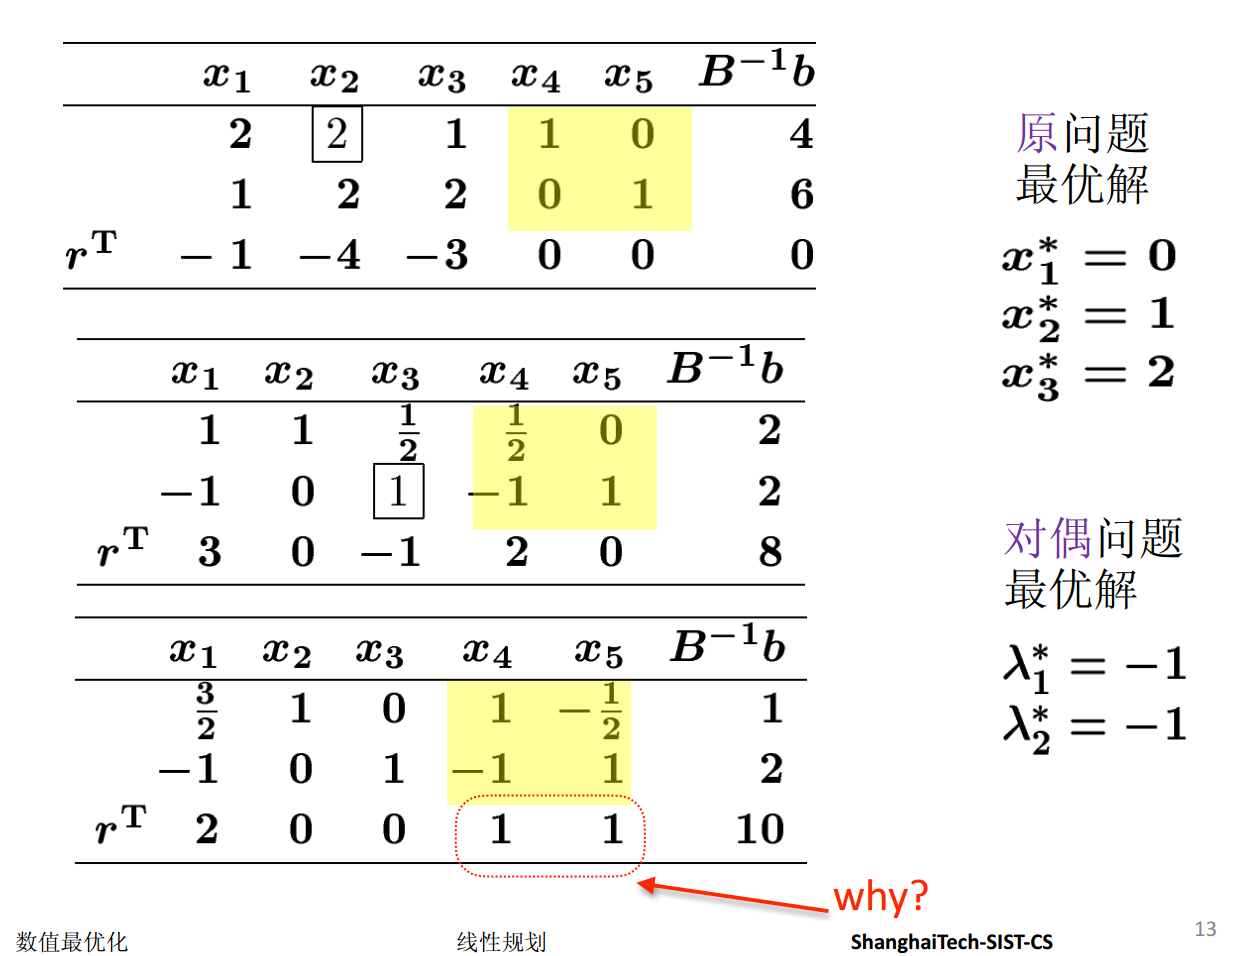
\includegraphics[width=4in]{pivot.jpg}
	\caption{Lecture $5$~第~$13$~页给出的单纯型表示例.}
	\label{fig: pivot}
\end{figure}\\
\textbf{解}\\
我们在单纯形表的最下行所存储的是reduced cost,定义是
$$r_j=c_j-c_B^TB^{-1}a_j$$
其中$c_j$代表着cost,$a_j$代表原矩阵的第$j$列。初始的单纯形表单位阵中的所有基变量对应的$c_{I} = 0, a_{I} = I$(下标$I$代表着由单位阵中变量对应的下标),因此我们进一步可以得到在最优变量对应基B下的reduced cost
	$$r_{I} = c_{I}-c_B^TB^{-1}a_{I} = -c_B^TB^{-1}$$
	即为最优的拉格朗日乘子的相反数。


$\bm{5}.$
证明: 线性规划问题求解等价于求解一个线性可行性问题.(\textcolor{red}{提示: 请参考~Lecture~$5$第~$14$页.})~\textcolor{red}{[15pts]}
\textbf{解}
首先我们先分别写出原对偶问题,原问题:
	\begin{equation}
		\begin{array}{ll}
			\min & c^Tx \\
			\text { s.t. } & Ax=b \\
			& x\ge 0
		\end{array}
	\end{equation}
对偶问题:
	\begin{equation}
		\begin{array}{ll}
			\min & b^Ty \\
			\text { s.t. } & A^Ty\le c 
		\end{array}
	\end{equation}
根据强对偶定理,原问题若有最优解,那么对偶问题也有最优解,并且最优值相等。即下述线性系统中要存在可行解
\begin{equation}
\begin{array}{ll}
	Ax &= b\\
	x&\ge 0 \\
	A^Ty+s&=c\\
	s&\ge 0\\
	b^Ty &=c^Tx
\end{array}
\end{equation}
由于$0=c^Tx-b^Ty=(c-A^Ty)^Tx=s^Tx$,因此上述线性系统等价于
\begin{equation}\label{ls}
	\begin{array}{ll}
	s^Tx &= 0\\
	s,x&\ge 0	
	\end{array}
\end{equation}
因此下面我们对是否存在最优解两种情况进行分类讨论
\begin{itemize}
	\item 若该线性规划问题有最优解,则对应\ref{ls}中存在一个可行解,该可行解即为原对偶问题中对偶间隙为0的一个最优解。
	\item 若该线规划问题没有最优解,则根据线性规划基本定理,原问题不存在一个可行解,此时\ref{ls}无法满足(不可能存在$b^Ty=c^Tx$,否则问题存在最优解),即\ref{ls}中无法找到一个可行解。
\end{itemize}
综上所述,线性规划问题等价于由原问题可行性条件、对偶问题可行性条件和互补条件组成的线性可行性问题。

\end{document}